\documentclass[12pt, french]{article}
\usepackage{graphicx} % insertion image
\usepackage{hyperref} % insertion liens
\usepackage{geometry} %insertion marge
\geometry{hmargin=3cm,vmargin=3.5cm}
\usepackage{ragged2e} % pour justifier le texte
\usepackage{setspace}
\setlength{\parindent}{30pt} 
\usepackage{amsmath}
\usepackage[ruled,vlined]{algorithm2e}
\usepackage{subcaption}
\usepackage{mdframed} 
\usepackage{bbold}



\usepackage[breakable]{tcolorbox}
    \usepackage{parskip} % Stop auto-indenting (to mimic markdown behaviour)
    

    % Basic figure setup, for now with no caption control since it's done
    % automatically by Pandoc (which extracts ![](path) syntax from Markdown).
    \usepackage{graphicx}
    % Maintain compatibility with old templates. Remove in nbconvert 6.0
    \let\Oldincludegraphics\includegraphics
    % Ensure that by default, figures have no caption (until we provide a
    % proper Figure object with a Caption API and a way to capture that
    % in the conversion process - todo).
    \usepackage{caption}
    \DeclareCaptionFormat{nocaption}{}
    \captionsetup{format=nocaption,aboveskip=0pt,belowskip=0pt}

    \usepackage{float}
    \floatplacement{figure}{H} % forces figures to be placed at the correct location
    \usepackage{xcolor} % Allow colors to be defined
    \usepackage{enumerate} % Needed for markdown enumerations to work
    \usepackage{geometry} % Used to adjust the document margins
    \usepackage{amsmath} % Equations
    \usepackage{amssymb} % Equations
    \usepackage{textcomp} % defines textquotesingle
    % Hack from http://tex.stackexchange.com/a/47451/13684:
    \AtBeginDocument{%
        \def\PYZsq{\textquotesingle}% Upright quotes in Pygmentized code
    }
    \usepackage{upquote} % Upright quotes for verbatim code
    \usepackage{eurosym} % defines \euro

    \usepackage{iftex}
    \ifPDFTeX
        \usepackage[T1]{fontenc}
        \IfFileExists{alphabeta.sty}{
              \usepackage{alphabeta}
          }{
              \usepackage[mathletters]{ucs}
              \usepackage[utf8x]{inputenc}
          }
    \else
        \usepackage{fontspec}
        \usepackage{unicode-math}
    \fi

    \usepackage{fancyvrb} % verbatim replacement that allows latex
    \usepackage{grffile} % extends the file name processing of package graphics
                         % to support a larger range
    \makeatletter % fix for old versions of grffile with XeLaTeX
    \@ifpackagelater{grffile}{2019/11/01}
    {
      % Do nothing on new versions
    }
    {
      \def\Gread@@xetex#1{%
        \IfFileExists{"\Gin@base".bb}%
        {\Gread@eps{\Gin@base.bb}}%
        {\Gread@@xetex@aux#1}%
      }
    }
    \makeatother
    \usepackage[Export]{adjustbox} % Used to constrain images to a maximum size
    \adjustboxset{max size={0.9\linewidth}{0.9\paperheight}}

    % The hyperref package gives us a pdf with properly built
    % internal navigation ('pdf bookmarks' for the table of contents,
    % internal cross-reference links, web links for URLs, etc.)
    \usepackage{hyperref}
    % The default LaTeX title has an obnoxious amount of whitespace. By default,
    % titling removes some of it. It also provides customization options.
    \usepackage{titling}
    \usepackage{longtable} % longtable support required by pandoc >1.10
    \usepackage{booktabs}  % table support for pandoc > 1.12.2
    \usepackage{array}     % table support for pandoc >= 2.11.3
    \usepackage{calc}      % table minipage width calculation for pandoc >= 2.11.1
    \usepackage[inline]{enumitem} % IRkernel/repr support (it uses the enumerate* environment)
    \usepackage[normalem]{ulem} % ulem is needed to support strikethroughs (\sout)
                                % normalem makes italics be italics, not underlines
    \usepackage{soul}      % strikethrough (\st) support for pandoc >= 3.0.0
    \usepackage{mathrsfs}
    

    
    % Colors for the hyperref package
    \definecolor{urlcolor}{rgb}{0,.145,.698}
    \definecolor{linkcolor}{rgb}{.71,0.21,0.01}
    \definecolor{citecolor}{rgb}{.12,.54,.11}

    % ANSI colors
    \definecolor{ansi-black}{HTML}{3E424D}
    \definecolor{ansi-black-intense}{HTML}{282C36}
    \definecolor{ansi-red}{HTML}{E75C58}
    \definecolor{ansi-red-intense}{HTML}{B22B31}
    \definecolor{ansi-green}{HTML}{00A250}
    \definecolor{ansi-green-intense}{HTML}{007427}
    \definecolor{ansi-yellow}{HTML}{DDB62B}
    \definecolor{ansi-yellow-intense}{HTML}{B27D12}
    \definecolor{ansi-blue}{HTML}{208FFB}
    \definecolor{ansi-blue-intense}{HTML}{0065CA}
    \definecolor{ansi-magenta}{HTML}{D160C4}
    \definecolor{ansi-magenta-intense}{HTML}{A03196}
    \definecolor{ansi-cyan}{HTML}{60C6C8}
    \definecolor{ansi-cyan-intense}{HTML}{258F8F}
    \definecolor{ansi-white}{HTML}{C5C1B4}
    \definecolor{ansi-white-intense}{HTML}{A1A6B2}
    \definecolor{ansi-default-inverse-fg}{HTML}{FFFFFF}
    \definecolor{ansi-default-inverse-bg}{HTML}{000000}

    % common color for the border for error outputs.
    \definecolor{outerrorbackground}{HTML}{FFDFDF}

    % commands and environments needed by pandoc snippets
    % extracted from the output of `pandoc -s`
    \providecommand{\tightlist}{%
      \setlength{\itemsep}{0pt}\setlength{\parskip}{0pt}}
    \DefineVerbatimEnvironment{Highlighting}{Verbatim}{commandchars=\\\{\}}
    % Add ',fontsize=\small' for more characters per line
    \newenvironment{Shaded}{}{}
    \newcommand{\KeywordTok}[1]{\textcolor[rgb]{0.00,0.44,0.13}{\textbf{{#1}}}}
    \newcommand{\DataTypeTok}[1]{\textcolor[rgb]{0.56,0.13,0.00}{{#1}}}
    \newcommand{\DecValTok}[1]{\textcolor[rgb]{0.25,0.63,0.44}{{#1}}}
    \newcommand{\BaseNTok}[1]{\textcolor[rgb]{0.25,0.63,0.44}{{#1}}}
    \newcommand{\FloatTok}[1]{\textcolor[rgb]{0.25,0.63,0.44}{{#1}}}
    \newcommand{\CharTok}[1]{\textcolor[rgb]{0.25,0.44,0.63}{{#1}}}
    \newcommand{\StringTok}[1]{\textcolor[rgb]{0.25,0.44,0.63}{{#1}}}
    \newcommand{\CommentTok}[1]{\textcolor[rgb]{0.38,0.63,0.69}{\textit{{#1}}}}
    \newcommand{\OtherTok}[1]{\textcolor[rgb]{0.00,0.44,0.13}{{#1}}}
    \newcommand{\AlertTok}[1]{\textcolor[rgb]{1.00,0.00,0.00}{\textbf{{#1}}}}
    \newcommand{\FunctionTok}[1]{\textcolor[rgb]{0.02,0.16,0.49}{{#1}}}
    \newcommand{\RegionMarkerTok}[1]{{#1}}
    \newcommand{\ErrorTok}[1]{\textcolor[rgb]{1.00,0.00,0.00}{\textbf{{#1}}}}
    \newcommand{\NormalTok}[1]{{#1}}

    % Additional commands for more recent versions of Pandoc
    \newcommand{\ConstantTok}[1]{\textcolor[rgb]{0.53,0.00,0.00}{{#1}}}
    \newcommand{\SpecialCharTok}[1]{\textcolor[rgb]{0.25,0.44,0.63}{{#1}}}
    \newcommand{\VerbatimStringTok}[1]{\textcolor[rgb]{0.25,0.44,0.63}{{#1}}}
    \newcommand{\SpecialStringTok}[1]{\textcolor[rgb]{0.73,0.40,0.53}{{#1}}}
    \newcommand{\ImportTok}[1]{{#1}}
    \newcommand{\DocumentationTok}[1]{\textcolor[rgb]{0.73,0.13,0.13}{\textit{{#1}}}}
    \newcommand{\AnnotationTok}[1]{\textcolor[rgb]{0.38,0.63,0.69}{\textbf{\textit{{#1}}}}}
    \newcommand{\CommentVarTok}[1]{\textcolor[rgb]{0.38,0.63,0.69}{\textbf{\textit{{#1}}}}}
    \newcommand{\VariableTok}[1]{\textcolor[rgb]{0.10,0.09,0.49}{{#1}}}
    \newcommand{\ControlFlowTok}[1]{\textcolor[rgb]{0.00,0.44,0.13}{\textbf{{#1}}}}
    \newcommand{\OperatorTok}[1]{\textcolor[rgb]{0.40,0.40,0.40}{{#1}}}
    \newcommand{\BuiltInTok}[1]{{#1}}
    \newcommand{\ExtensionTok}[1]{{#1}}
    \newcommand{\PreprocessorTok}[1]{\textcolor[rgb]{0.74,0.48,0.00}{{#1}}}
    \newcommand{\AttributeTok}[1]{\textcolor[rgb]{0.49,0.56,0.16}{{#1}}}
    \newcommand{\InformationTok}[1]{\textcolor[rgb]{0.38,0.63,0.69}{\textbf{\textit{{#1}}}}}
    \newcommand{\WarningTok}[1]{\textcolor[rgb]{0.38,0.63,0.69}{\textbf{\textit{{#1}}}}}


    % Define a nice break command that doesn't care if a line doesn't already
    % exist.
    \def\br{\hspace*{\fill} \\* }
    % Math Jax compatibility definitions
    \def\gt{>}
    \def\lt{<}
    \let\Oldtex\TeX
    \let\Oldlatex\LaTeX
    \renewcommand{\TeX}{\textrm{\Oldtex}}
    \renewcommand{\LaTeX}{\textrm{\Oldlatex}}
    % Document parameters
    % Document title
    \title{main}
    
    
    
    
    
    
    
% Pygments definitions
\makeatletter
\def\PY@reset{\let\PY@it=\relax \let\PY@bf=\relax%
    \let\PY@ul=\relax \let\PY@tc=\relax%
    \let\PY@bc=\relax \let\PY@ff=\relax}
\def\PY@tok#1{\csname PY@tok@#1\endcsname}
\def\PY@toks#1+{\ifx\relax#1\empty\else%
    \PY@tok{#1}\expandafter\PY@toks\fi}
\def\PY@do#1{\PY@bc{\PY@tc{\PY@ul{%
    \PY@it{\PY@bf{\PY@ff{#1}}}}}}}
\def\PY#1#2{\PY@reset\PY@toks#1+\relax+\PY@do{#2}}

\@namedef{PY@tok@w}{\def\PY@tc##1{\textcolor[rgb]{0.73,0.73,0.73}{##1}}}
\@namedef{PY@tok@c}{\let\PY@it=\textit\def\PY@tc##1{\textcolor[rgb]{0.24,0.48,0.48}{##1}}}
\@namedef{PY@tok@cp}{\def\PY@tc##1{\textcolor[rgb]{0.61,0.40,0.00}{##1}}}
\@namedef{PY@tok@k}{\let\PY@bf=\textbf\def\PY@tc##1{\textcolor[rgb]{0.00,0.50,0.00}{##1}}}
\@namedef{PY@tok@kp}{\def\PY@tc##1{\textcolor[rgb]{0.00,0.50,0.00}{##1}}}
\@namedef{PY@tok@kt}{\def\PY@tc##1{\textcolor[rgb]{0.69,0.00,0.25}{##1}}}
\@namedef{PY@tok@o}{\def\PY@tc##1{\textcolor[rgb]{0.40,0.40,0.40}{##1}}}
\@namedef{PY@tok@ow}{\let\PY@bf=\textbf\def\PY@tc##1{\textcolor[rgb]{0.67,0.13,1.00}{##1}}}
\@namedef{PY@tok@nb}{\def\PY@tc##1{\textcolor[rgb]{0.00,0.50,0.00}{##1}}}
\@namedef{PY@tok@nf}{\def\PY@tc##1{\textcolor[rgb]{0.00,0.00,1.00}{##1}}}
\@namedef{PY@tok@nc}{\let\PY@bf=\textbf\def\PY@tc##1{\textcolor[rgb]{0.00,0.00,1.00}{##1}}}
\@namedef{PY@tok@nn}{\let\PY@bf=\textbf\def\PY@tc##1{\textcolor[rgb]{0.00,0.00,1.00}{##1}}}
\@namedef{PY@tok@ne}{\let\PY@bf=\textbf\def\PY@tc##1{\textcolor[rgb]{0.80,0.25,0.22}{##1}}}
\@namedef{PY@tok@nv}{\def\PY@tc##1{\textcolor[rgb]{0.10,0.09,0.49}{##1}}}
\@namedef{PY@tok@no}{\def\PY@tc##1{\textcolor[rgb]{0.53,0.00,0.00}{##1}}}
\@namedef{PY@tok@nl}{\def\PY@tc##1{\textcolor[rgb]{0.46,0.46,0.00}{##1}}}
\@namedef{PY@tok@ni}{\let\PY@bf=\textbf\def\PY@tc##1{\textcolor[rgb]{0.44,0.44,0.44}{##1}}}
\@namedef{PY@tok@na}{\def\PY@tc##1{\textcolor[rgb]{0.41,0.47,0.13}{##1}}}
\@namedef{PY@tok@nt}{\let\PY@bf=\textbf\def\PY@tc##1{\textcolor[rgb]{0.00,0.50,0.00}{##1}}}
\@namedef{PY@tok@nd}{\def\PY@tc##1{\textcolor[rgb]{0.67,0.13,1.00}{##1}}}
\@namedef{PY@tok@s}{\def\PY@tc##1{\textcolor[rgb]{0.73,0.13,0.13}{##1}}}
\@namedef{PY@tok@sd}{\let\PY@it=\textit\def\PY@tc##1{\textcolor[rgb]{0.73,0.13,0.13}{##1}}}
\@namedef{PY@tok@si}{\let\PY@bf=\textbf\def\PY@tc##1{\textcolor[rgb]{0.64,0.35,0.47}{##1}}}
\@namedef{PY@tok@se}{\let\PY@bf=\textbf\def\PY@tc##1{\textcolor[rgb]{0.67,0.36,0.12}{##1}}}
\@namedef{PY@tok@sr}{\def\PY@tc##1{\textcolor[rgb]{0.64,0.35,0.47}{##1}}}
\@namedef{PY@tok@ss}{\def\PY@tc##1{\textcolor[rgb]{0.10,0.09,0.49}{##1}}}
\@namedef{PY@tok@sx}{\def\PY@tc##1{\textcolor[rgb]{0.00,0.50,0.00}{##1}}}
\@namedef{PY@tok@m}{\def\PY@tc##1{\textcolor[rgb]{0.40,0.40,0.40}{##1}}}
\@namedef{PY@tok@gh}{\let\PY@bf=\textbf\def\PY@tc##1{\textcolor[rgb]{0.00,0.00,0.50}{##1}}}
\@namedef{PY@tok@gu}{\let\PY@bf=\textbf\def\PY@tc##1{\textcolor[rgb]{0.50,0.00,0.50}{##1}}}
\@namedef{PY@tok@gd}{\def\PY@tc##1{\textcolor[rgb]{0.63,0.00,0.00}{##1}}}
\@namedef{PY@tok@gi}{\def\PY@tc##1{\textcolor[rgb]{0.00,0.52,0.00}{##1}}}
\@namedef{PY@tok@gr}{\def\PY@tc##1{\textcolor[rgb]{0.89,0.00,0.00}{##1}}}
\@namedef{PY@tok@ge}{\let\PY@it=\textit}
\@namedef{PY@tok@gs}{\let\PY@bf=\textbf}
\@namedef{PY@tok@ges}{\let\PY@bf=\textbf\let\PY@it=\textit}
\@namedef{PY@tok@gp}{\let\PY@bf=\textbf\def\PY@tc##1{\textcolor[rgb]{0.00,0.00,0.50}{##1}}}
\@namedef{PY@tok@go}{\def\PY@tc##1{\textcolor[rgb]{0.44,0.44,0.44}{##1}}}
\@namedef{PY@tok@gt}{\def\PY@tc##1{\textcolor[rgb]{0.00,0.27,0.87}{##1}}}
\@namedef{PY@tok@err}{\def\PY@bc##1{{\setlength{\fboxsep}{\string -\fboxrule}\fcolorbox[rgb]{1.00,0.00,0.00}{1,1,1}{\strut ##1}}}}
\@namedef{PY@tok@kc}{\let\PY@bf=\textbf\def\PY@tc##1{\textcolor[rgb]{0.00,0.50,0.00}{##1}}}
\@namedef{PY@tok@kd}{\let\PY@bf=\textbf\def\PY@tc##1{\textcolor[rgb]{0.00,0.50,0.00}{##1}}}
\@namedef{PY@tok@kn}{\let\PY@bf=\textbf\def\PY@tc##1{\textcolor[rgb]{0.00,0.50,0.00}{##1}}}
\@namedef{PY@tok@kr}{\let\PY@bf=\textbf\def\PY@tc##1{\textcolor[rgb]{0.00,0.50,0.00}{##1}}}
\@namedef{PY@tok@bp}{\def\PY@tc##1{\textcolor[rgb]{0.00,0.50,0.00}{##1}}}
\@namedef{PY@tok@fm}{\def\PY@tc##1{\textcolor[rgb]{0.00,0.00,1.00}{##1}}}
\@namedef{PY@tok@vc}{\def\PY@tc##1{\textcolor[rgb]{0.10,0.09,0.49}{##1}}}
\@namedef{PY@tok@vg}{\def\PY@tc##1{\textcolor[rgb]{0.10,0.09,0.49}{##1}}}
\@namedef{PY@tok@vi}{\def\PY@tc##1{\textcolor[rgb]{0.10,0.09,0.49}{##1}}}
\@namedef{PY@tok@vm}{\def\PY@tc##1{\textcolor[rgb]{0.10,0.09,0.49}{##1}}}
\@namedef{PY@tok@sa}{\def\PY@tc##1{\textcolor[rgb]{0.73,0.13,0.13}{##1}}}
\@namedef{PY@tok@sb}{\def\PY@tc##1{\textcolor[rgb]{0.73,0.13,0.13}{##1}}}
\@namedef{PY@tok@sc}{\def\PY@tc##1{\textcolor[rgb]{0.73,0.13,0.13}{##1}}}
\@namedef{PY@tok@dl}{\def\PY@tc##1{\textcolor[rgb]{0.73,0.13,0.13}{##1}}}
\@namedef{PY@tok@s2}{\def\PY@tc##1{\textcolor[rgb]{0.73,0.13,0.13}{##1}}}
\@namedef{PY@tok@sh}{\def\PY@tc##1{\textcolor[rgb]{0.73,0.13,0.13}{##1}}}
\@namedef{PY@tok@s1}{\def\PY@tc##1{\textcolor[rgb]{0.73,0.13,0.13}{##1}}}
\@namedef{PY@tok@mb}{\def\PY@tc##1{\textcolor[rgb]{0.40,0.40,0.40}{##1}}}
\@namedef{PY@tok@mf}{\def\PY@tc##1{\textcolor[rgb]{0.40,0.40,0.40}{##1}}}
\@namedef{PY@tok@mh}{\def\PY@tc##1{\textcolor[rgb]{0.40,0.40,0.40}{##1}}}
\@namedef{PY@tok@mi}{\def\PY@tc##1{\textcolor[rgb]{0.40,0.40,0.40}{##1}}}
\@namedef{PY@tok@il}{\def\PY@tc##1{\textcolor[rgb]{0.40,0.40,0.40}{##1}}}
\@namedef{PY@tok@mo}{\def\PY@tc##1{\textcolor[rgb]{0.40,0.40,0.40}{##1}}}
\@namedef{PY@tok@ch}{\let\PY@it=\textit\def\PY@tc##1{\textcolor[rgb]{0.24,0.48,0.48}{##1}}}
\@namedef{PY@tok@cm}{\let\PY@it=\textit\def\PY@tc##1{\textcolor[rgb]{0.24,0.48,0.48}{##1}}}
\@namedef{PY@tok@cpf}{\let\PY@it=\textit\def\PY@tc##1{\textcolor[rgb]{0.24,0.48,0.48}{##1}}}
\@namedef{PY@tok@c1}{\let\PY@it=\textit\def\PY@tc##1{\textcolor[rgb]{0.24,0.48,0.48}{##1}}}
\@namedef{PY@tok@cs}{\let\PY@it=\textit\def\PY@tc##1{\textcolor[rgb]{0.24,0.48,0.48}{##1}}}

\def\PYZbs{\char`\\}
\def\PYZus{\char`\_}
\def\PYZob{\char`\{}
\def\PYZcb{\char`\}}
\def\PYZca{\char`\^}
\def\PYZam{\char`\&}
\def\PYZlt{\char`\<}
\def\PYZgt{\char`\>}
\def\PYZsh{\char`\#}
\def\PYZpc{\char`\%}
\def\PYZdl{\char`\$}
\def\PYZhy{\char`\-}
\def\PYZsq{\char`\'}
\def\PYZdq{\char`\"}
\def\PYZti{\char`\~}
% for compatibility with earlier versions
\def\PYZat{@}
\def\PYZlb{[}
\def\PYZrb{]}
\makeatother


    % For linebreaks inside Verbatim environment from package fancyvrb.
    \makeatletter
        \newbox\Wrappedcontinuationbox
        \newbox\Wrappedvisiblespacebox
        \newcommand*\Wrappedvisiblespace {\textcolor{red}{\textvisiblespace}}
        \newcommand*\Wrappedcontinuationsymbol {\textcolor{red}{\llap{\tiny$\m@th\hookrightarrow$}}}
        \newcommand*\Wrappedcontinuationindent {3ex }
        \newcommand*\Wrappedafterbreak {\kern\Wrappedcontinuationindent\copy\Wrappedcontinuationbox}
        % Take advantage of the already applied Pygments mark-up to insert
        % potential linebreaks for TeX processing.
        %        {, <, #, %, $, ' and ": go to next line.
        %        _, }, ^, &, >, - and ~: stay at end of broken line.
        % Use of \textquotesingle for straight quote.
        \newcommand*\Wrappedbreaksatspecials {%
            \def\PYGZus{\discretionary{\char`\_}{\Wrappedafterbreak}{\char`\_}}%
            \def\PYGZob{\discretionary{}{\Wrappedafterbreak\char`\{}{\char`\{}}%
            \def\PYGZcb{\discretionary{\char`\}}{\Wrappedafterbreak}{\char`\}}}%
            \def\PYGZca{\discretionary{\char`\^}{\Wrappedafterbreak}{\char`\^}}%
            \def\PYGZam{\discretionary{\char`\&}{\Wrappedafterbreak}{\char`\&}}%
            \def\PYGZlt{\discretionary{}{\Wrappedafterbreak\char`\<}{\char`\<}}%
            \def\PYGZgt{\discretionary{\char`\>}{\Wrappedafterbreak}{\char`\>}}%
            \def\PYGZsh{\discretionary{}{\Wrappedafterbreak\char`\#}{\char`\#}}%
            \def\PYGZpc{\discretionary{}{\Wrappedafterbreak\char`\%}{\char`\%}}%
            \def\PYGZdl{\discretionary{}{\Wrappedafterbreak\char`\$}{\char`\$}}%
            \def\PYGZhy{\discretionary{\char`\-}{\Wrappedafterbreak}{\char`\-}}%
            \def\PYGZsq{\discretionary{}{\Wrappedafterbreak\textquotesingle}{\textquotesingle}}%
            \def\PYGZdq{\discretionary{}{\Wrappedafterbreak\char`\"}{\char`\"}}%
            \def\PYGZti{\discretionary{\char`\~}{\Wrappedafterbreak}{\char`\~}}%
        }
        % Some characters . , ; ? ! / are not pygmentized.
        % This macro makes them "active" and they will insert potential linebreaks
        \newcommand*\Wrappedbreaksatpunct {%
            \lccode`\~`\.\lowercase{\def~}{\discretionary{\hbox{\char`\.}}{\Wrappedafterbreak}{\hbox{\char`\.}}}%
            \lccode`\~`\,\lowercase{\def~}{\discretionary{\hbox{\char`\,}}{\Wrappedafterbreak}{\hbox{\char`\,}}}%
            \lccode`\~`\;\lowercase{\def~}{\discretionary{\hbox{\char`\;}}{\Wrappedafterbreak}{\hbox{\char`\;}}}%
            \lccode`\~`\:\lowercase{\def~}{\discretionary{\hbox{\char`\:}}{\Wrappedafterbreak}{\hbox{\char`\:}}}%
            \lccode`\~`\?\lowercase{\def~}{\discretionary{\hbox{\char`\?}}{\Wrappedafterbreak}{\hbox{\char`\?}}}%
            \lccode`\~`\!\lowercase{\def~}{\discretionary{\hbox{\char`\!}}{\Wrappedafterbreak}{\hbox{\char`\!}}}%
            \lccode`\~`\/\lowercase{\def~}{\discretionary{\hbox{\char`\/}}{\Wrappedafterbreak}{\hbox{\char`\/}}}%
            \catcode`\.\active
            \catcode`\,\active
            \catcode`\;\active
            \catcode`\:\active
            \catcode`\?\active
            \catcode`\!\active
            \catcode`\/\active
            \lccode`\~`\~
        }
    \makeatother

    \let\OriginalVerbatim=\Verbatim
    \makeatletter
    \renewcommand{\Verbatim}[1][1]{%
        %\parskip\z@skip
        \sbox\Wrappedcontinuationbox {\Wrappedcontinuationsymbol}%
        \sbox\Wrappedvisiblespacebox {\FV@SetupFont\Wrappedvisiblespace}%
        \def\FancyVerbFormatLine ##1{\hsize\linewidth
            \vtop{\raggedright\hyphenpenalty\z@\exhyphenpenalty\z@
                \doublehyphendemerits\z@\finalhyphendemerits\z@
                \strut ##1\strut}%
        }%
        % If the linebreak is at a space, the latter will be displayed as visible
        % space at end of first line, and a continuation symbol starts next line.
        % Stretch/shrink are however usually zero for typewriter font.
        \def\FV@Space {%
            \nobreak\hskip\z@ plus\fontdimen3\font minus\fontdimen4\font
            \discretionary{\copy\Wrappedvisiblespacebox}{\Wrappedafterbreak}
            {\kern\fontdimen2\font}%
        }%

        % Allow breaks at special characters using \PYG... macros.
        \Wrappedbreaksatspecials
        % Breaks at punctuation characters . , ; ? ! and / need catcode=\active
        \OriginalVerbatim[#1,codes*=\Wrappedbreaksatpunct]%
    }
    \makeatother

    % Exact colors from NB
    \definecolor{incolor}{HTML}{303F9F}
    \definecolor{outcolor}{HTML}{D84315}
    \definecolor{cellborder}{HTML}{CFCFCF}
    \definecolor{cellbackground}{HTML}{F7F7F7}

    % prompt
    \makeatletter
    \newcommand{\boxspacing}{\kern\kvtcb@left@rule\kern\kvtcb@boxsep}
    \makeatother
    \newcommand{\prompt}[4]{
        {\ttfamily\llap{{\color{#2}[#3]:\hspace{3pt}#4}}\vspace{-\baselineskip}}
    }
    

    
    % Prevent overflowing lines due to hard-to-break entities
    \sloppy
    % Setup hyperref package
    \hypersetup{
      breaklinks=true,  % so long urls are correctly broken across lines
      colorlinks=true,
      urlcolor=urlcolor,
      linkcolor=linkcolor,
      citecolor=citecolor,
      }
    % Slightly bigger margins than the latex defaults
    
    \geometry{verbose,tmargin=1in,bmargin=1in,lmargin=1in,rmargin=1in}



    


\title{\textbf{Projet SQL \\ Requêtes Sakila -- Technique en Entreprise}}
\vspace{5cm}
\author{Hoang Thuy Duong Vu \\
        Johan Ghré \\
        Céline Chen \\
        Inès Hummel}
\date{Octobre 2024}

\AtBeginDocument{\renewcommand{\contentsname}{Table de matière}}

\begin{document}
\onehalfspacing
\justifying
\maketitle
\thispagestyle{empty}

\vfill
\begin{center}
    Projet réalisé sous la direction de M. Benoît Grand
\end{center}


\begin{figure}[!t] 
    \centering
    \includegraphics[width=0.5\textwidth]{logo-pantheon-sorbonne.png}
    \label{Panthéon Sorbonne}
\end{figure}

\vfill
\begin{center}
\href{https://github.com/Meriadoc-gitgit/SQL-SDA24}{Code source du Projet}
\end{center}

\newpage
\tableofcontents

\newpage

    

\section{1ère partie -- Base de données
Sakila}\label{uxe8re-partie-base-de-donnuxe9es-sakila}

\begin{enumerate}
\def\labelenumi{\arabic{enumi}.}
\tightlist
\item
  Tous les acteurs dont le nom de famille contient les lettres `gen'
\end{enumerate}

\begin{Shaded}
\begin{Highlighting}[]
\KeywordTok{select} \OperatorTok{*} \KeywordTok{from}\NormalTok{ sakila.actor}
\KeywordTok{where} \FunctionTok{lower}\NormalTok{(last\_name) }\KeywordTok{like} \StringTok{\textquotesingle{}\%gen\%\textquotesingle{}}\NormalTok{;}
\end{Highlighting}
\end{Shaded}

\begin{figure}[H] % Use [H] to enforce positioning
    \centering
    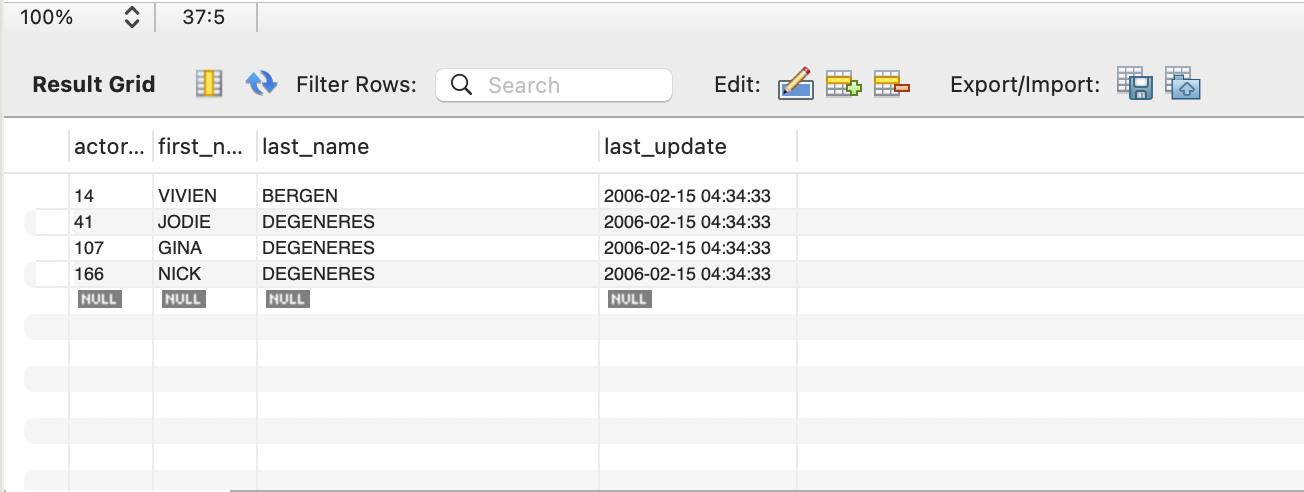
\includegraphics[width=0.75\textwidth]{res/Q1.png}
    \caption{Results of SQL Query for Actors with 'gen' in Last Name}
    \label{fig:actors_with_gen}
\end{figure}



\begin{enumerate}
\def\labelenumi{\arabic{enumi}.}
\setcounter{enumi}{1}
\tightlist
\item
  Tous les acteurs dont le nom de famille contient les lettres `li'
\end{enumerate}

\begin{Shaded}
\begin{Highlighting}[]
\KeywordTok{select} \OperatorTok{*} \KeywordTok{from}\NormalTok{ sakila.actor}
\KeywordTok{where} \FunctionTok{lower}\NormalTok{(last\_name) }\KeywordTok{like} \StringTok{\textquotesingle{}\%li\%\textquotesingle{}}\NormalTok{;}
\end{Highlighting}
\end{Shaded}

\begin{figure}[H] % Use [H] to enforce positioning
    \centering
    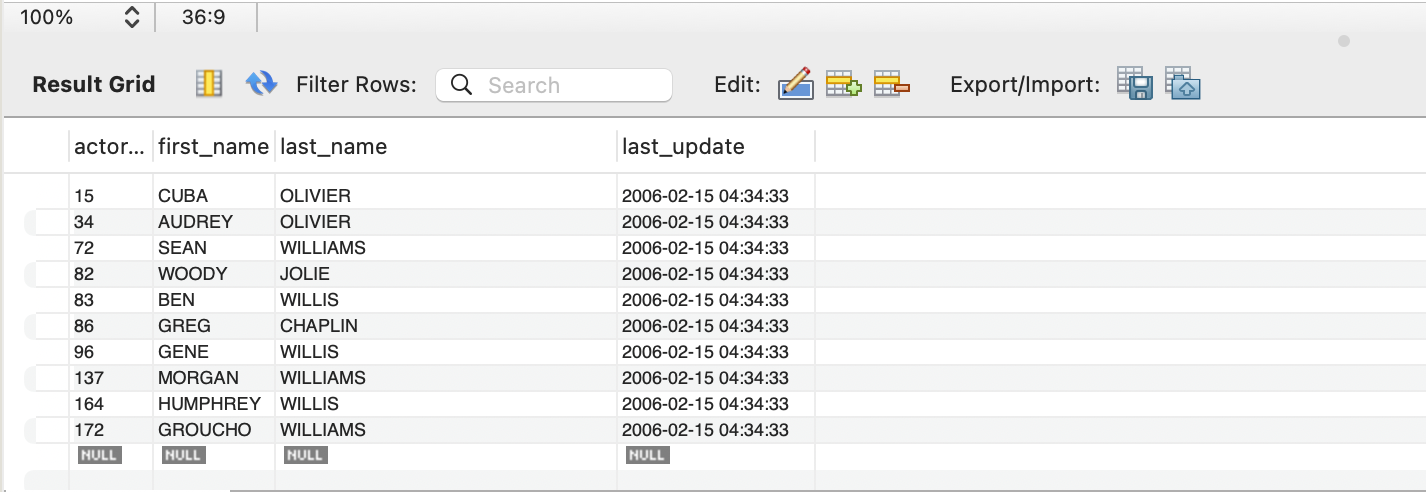
\includegraphics[width=0.75\textwidth]{res/Q2.png}
    \caption{Results of SQL Query for Actors with 'gen' in Last Name}
    \label{fig:actors_with_gen}
\end{figure}

\begin{enumerate}
\def\labelenumi{\arabic{enumi}.}
\setcounter{enumi}{2}
\tightlist
\item
  Liste des noms de famille de tous les acteurs, ainsi que le nombre
  d'acteurs portant chaque nom de famille
\end{enumerate}

\begin{Shaded}
\begin{Highlighting}[]
\KeywordTok{select}\NormalTok{ last\_name, }\FunctionTok{count}\NormalTok{(}\OperatorTok{*}\NormalTok{)}
\KeywordTok{from}\NormalTok{ sakila.actor}
\KeywordTok{group} \KeywordTok{by}\NormalTok{ last\_name;}
\end{Highlighting}
\end{Shaded}

\begin{figure}[H] % Use [H] to enforce positioning
    \centering
    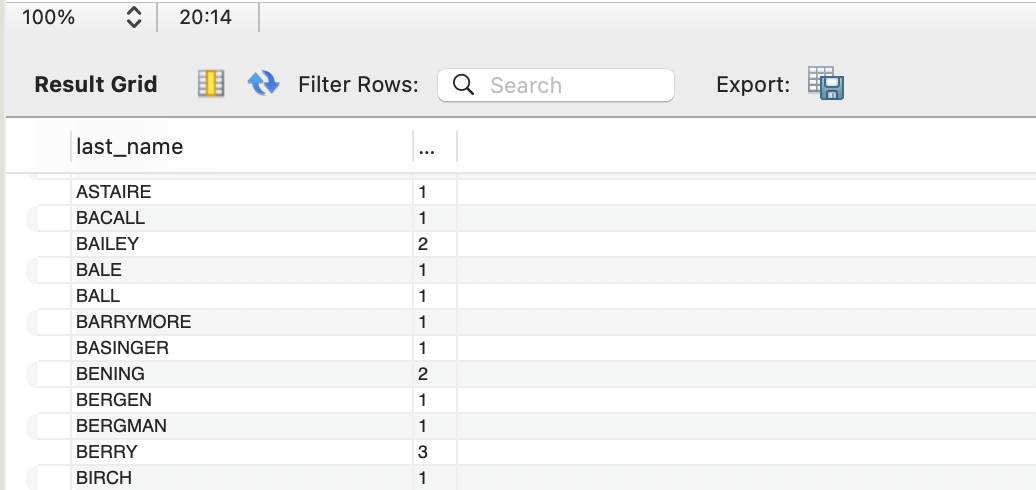
\includegraphics[width=0.75\textwidth]{res/Q3.png}
    \caption{Results of SQL Query for Actors with 'gen' in Last Name}
    \label{fig:actors_with_gen}
\end{figure}


\begin{enumerate}
\def\labelenumi{\arabic{enumi}.}
\setcounter{enumi}{3}
\tightlist
\item
  Liste des noms de famille des acteurs et le nombre d'acteurs qui
  portent chaque nom de famille, mais seulement pour les noms qui sont
  portés par au moins 2 acteurs
\end{enumerate}

\begin{Shaded}
\begin{Highlighting}[]
\KeywordTok{select}\NormalTok{ last\_name, }\FunctionTok{count}\NormalTok{(}\OperatorTok{*}\NormalTok{)}
\KeywordTok{from}\NormalTok{ sakila.actor}
\KeywordTok{group} \KeywordTok{by}\NormalTok{ last\_name }
\KeywordTok{having} \FunctionTok{count}\NormalTok{(}\OperatorTok{*}\NormalTok{) }\OperatorTok{\textgreater{}=} \DecValTok{2}\NormalTok{;}
\end{Highlighting}
\end{Shaded}


\begin{figure}[H] % Use [H] to enforce positioning
    \centering
    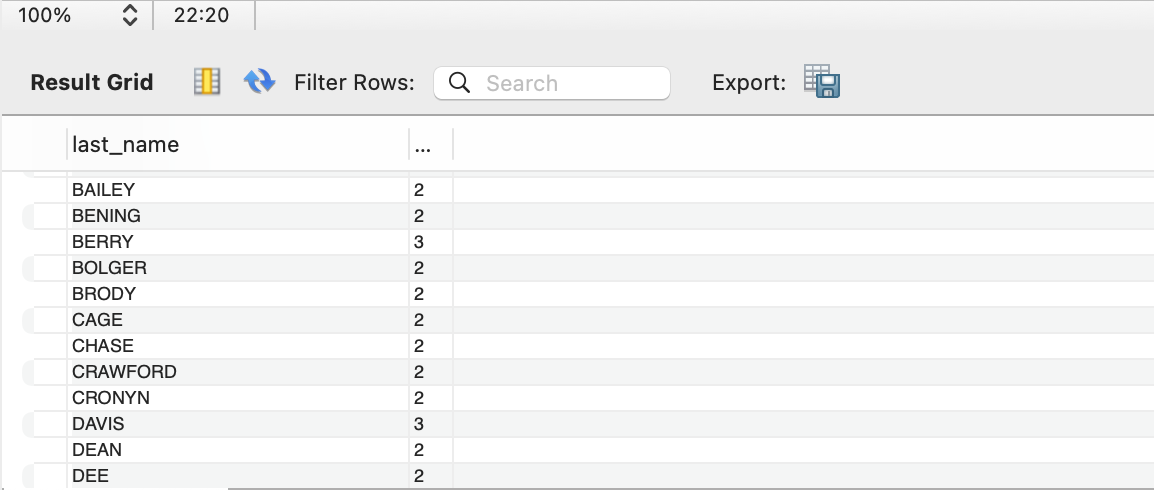
\includegraphics[width=0.75\textwidth]{res/Q4.png}
    \caption{Results of SQL Query for Actors with 'gen' in Last Name}
    \label{fig:actors_with_gen}
\end{figure}


\begin{enumerate}
\def\labelenumi{\arabic{enumi}.}
\setcounter{enumi}{4}
\tightlist
\item
  Utilisez JOIN pour afficher le montant total perçu par chaque membre
  du personnel en août 2005
\end{enumerate}

\begin{Shaded}
\begin{Highlighting}[]
\KeywordTok{select}\NormalTok{ p.staff\_id, s.first\_name, s.last\_name, }\FunctionTok{sum}\NormalTok{(p.amount)}
\KeywordTok{from}\NormalTok{ sakila.staff s }\KeywordTok{join}\NormalTok{ sakila.payment p }\KeywordTok{on}\NormalTok{ s.staff\_id }\OperatorTok{=}\NormalTok{ p.staff\_id}
\KeywordTok{where}\NormalTok{ date\_format(p.payment\_date, }\StringTok{\textquotesingle{}\%Y{-}\%m\textquotesingle{}}\NormalTok{) }\OperatorTok{=} \StringTok{\textquotesingle{}2005{-}08\textquotesingle{}}
\KeywordTok{group} \KeywordTok{by}\NormalTok{ p.staff\_id, s.first\_name, s.last\_name;}
\end{Highlighting}
\end{Shaded}


\begin{figure}[H] % Use [H] to enforce positioning
    \centering
    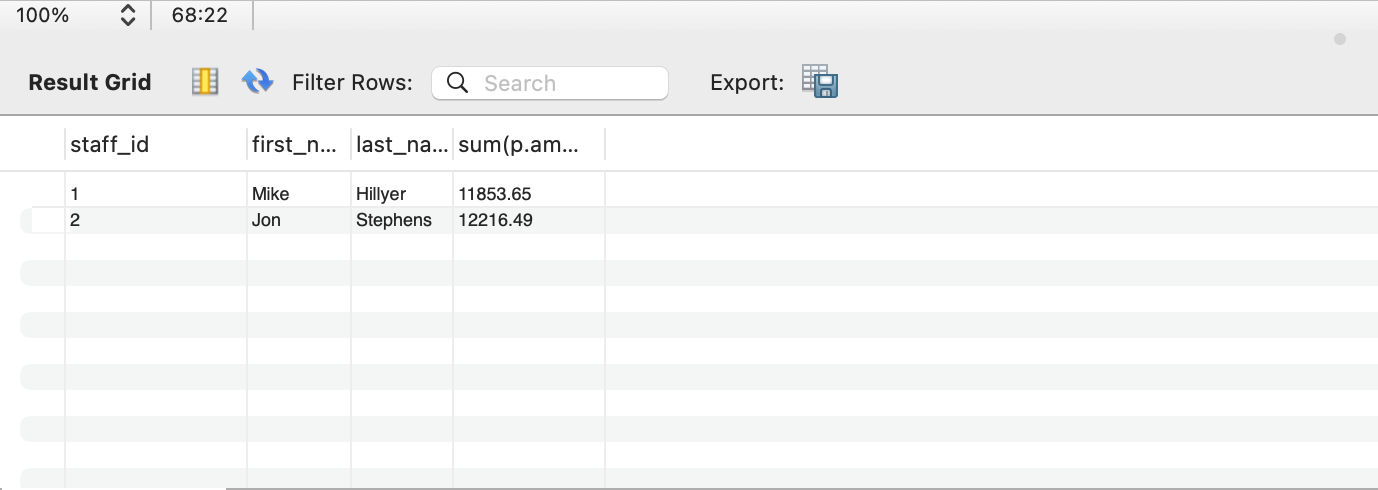
\includegraphics[width=0.75\textwidth]{res/Q5.png}
    \caption{Results of SQL Query for Actors with 'gen' in Last Name}
    \label{fig:actors_with_gen}
\end{figure}


\begin{enumerate}
\def\labelenumi{\arabic{enumi}.}
\setcounter{enumi}{5}
\tightlist
\item
  Afficher les titres des films commençant par les lettres K et Q dont
  la langue est l'anglais
\end{enumerate}

\begin{Shaded}
\begin{Highlighting}[]
\KeywordTok{select} \KeywordTok{distinct}\NormalTok{ f.title}
\KeywordTok{from}\NormalTok{ sakila.film f, sakila.language l}
\KeywordTok{where} 
    \FunctionTok{lower}\NormalTok{(f.title) }\KeywordTok{like} \StringTok{\textquotesingle{}k\%\textquotesingle{}} \KeywordTok{or} \FunctionTok{lower}\NormalTok{(f.title) }\KeywordTok{like} \StringTok{\textquotesingle{}q\%\textquotesingle{}}
    \KeywordTok{and}\NormalTok{ f.language\_id }\OperatorTok{=}\NormalTok{ l.language\_id }\KeywordTok{and}\NormalTok{ l.name }\OperatorTok{=} \StringTok{\textquotesingle{}English\textquotesingle{}}\NormalTok{;}
\end{Highlighting}
\end{Shaded}

\begin{figure}[H] % Use [H] to enforce positioning
    \centering
    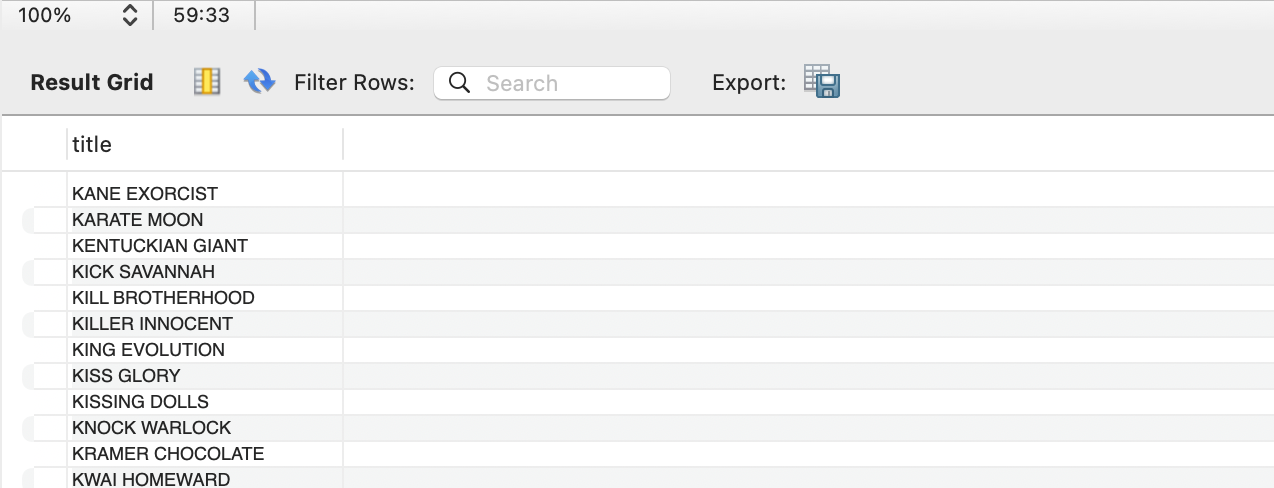
\includegraphics[width=0.75\textwidth]{res/Q6.png}
    \caption{Results of SQL Query for Actors with 'gen' in Last Name}
    \label{fig:actors_with_gen}
\end{figure}


\begin{enumerate}
\def\labelenumi{\arabic{enumi}.}
\setcounter{enumi}{6}
\tightlist
\item
  Affichez les noms et les adresses électroniques de tous les clients
  canadiens
\end{enumerate}

\begin{Shaded}
\begin{Highlighting}[]
\KeywordTok{select}\NormalTok{ c.last\_name, c.email, c.email, a.address, a.district, ci.city, a.postal\_code, co.country }
\KeywordTok{from}\NormalTok{ sakila.customer c, sakila.city ci, sakila.address a, sakila.country co}
\KeywordTok{where} 
\NormalTok{    c.address\_id }\OperatorTok{=}\NormalTok{ a.address\_id }\KeywordTok{and}\NormalTok{ ci.city\_id }\OperatorTok{=}\NormalTok{ a.city\_id }
    \KeywordTok{and}\NormalTok{ co.country\_id }\OperatorTok{=}\NormalTok{ ci.country\_id }\KeywordTok{and}\NormalTok{ co.country }\OperatorTok{=} \StringTok{\textquotesingle{}Canada\textquotesingle{}}\NormalTok{;}
\end{Highlighting}
\end{Shaded}

\begin{figure}[H] % Use [H] to enforce positioning
    \centering
    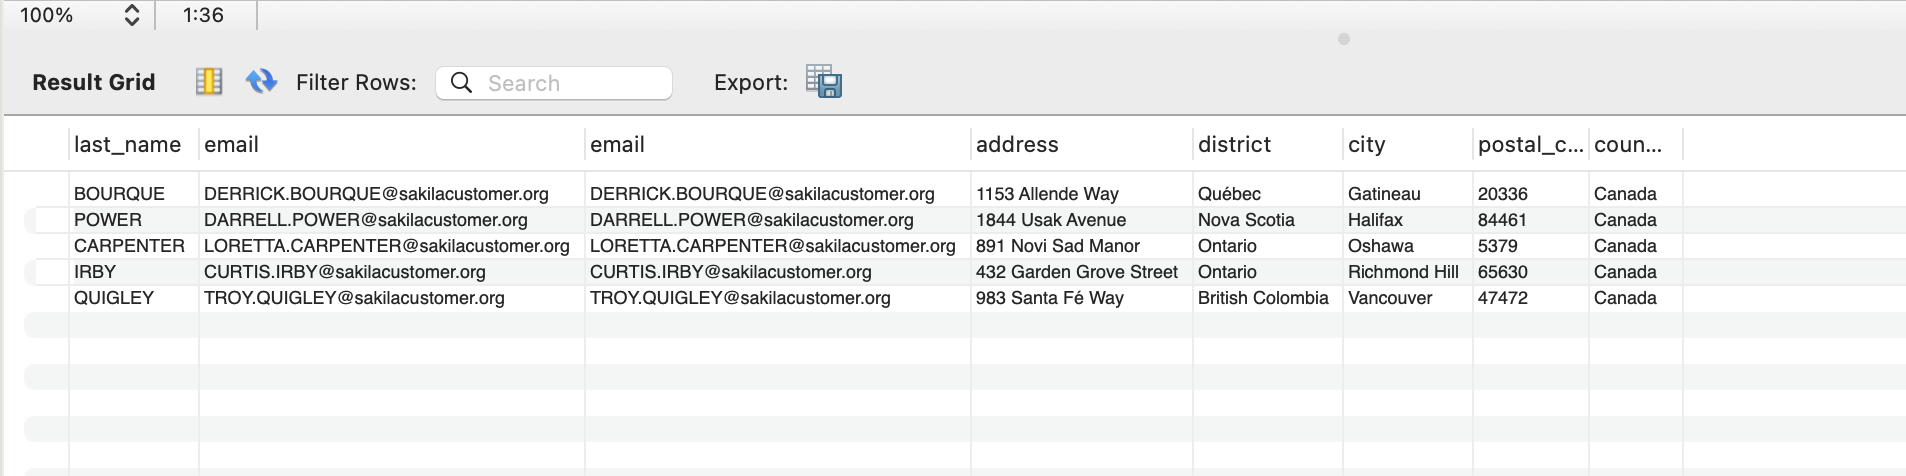
\includegraphics[width=0.75\textwidth]{res/Q7.png}
    \caption{Results of SQL Query for Actors with 'gen' in Last Name}
    \label{fig:actors_with_gen}
\end{figure}

\begin{enumerate}
\def\labelenumi{\arabic{enumi}.}
\setcounter{enumi}{7}
\tightlist
\item
  Quelles sont les ventes de chaque magasin pour chaque mois de 2005
  (CONCAT)
\end{enumerate}

\begin{Shaded}
\begin{Highlighting}[]
\KeywordTok{select}\NormalTok{ s.store\_id, }\FunctionTok{count}\NormalTok{(p.payment\_id) }\KeywordTok{as}\NormalTok{ number\_sold, }\FunctionTok{concat}\NormalTok{(}\StringTok{\textquotesingle{}0\textquotesingle{}}\NormalTok{,}\DataTypeTok{month}\NormalTok{(p.payment\_date),}\StringTok{\textquotesingle{}{-}\textquotesingle{}}\NormalTok{,}\DataTypeTok{year}\NormalTok{(p.payment\_date)) }\KeywordTok{as}\NormalTok{ month\_year}
\KeywordTok{from}\NormalTok{ sakila.payment p, sakila.staff st, sakila.}\KeywordTok{store}\NormalTok{ s}
\KeywordTok{where} 
\NormalTok{    p.staff\_id }\OperatorTok{=}\NormalTok{ st.staff\_id }
    \KeywordTok{and}\NormalTok{ st.store\_id }\OperatorTok{=}\NormalTok{ s.store\_id}
    \KeywordTok{and} \DataTypeTok{year}\NormalTok{(p.payment\_date) }\OperatorTok{=} \DecValTok{2005}
\KeywordTok{group} \KeywordTok{by} \FunctionTok{concat}\NormalTok{(}\StringTok{\textquotesingle{}0\textquotesingle{}}\NormalTok{,}\DataTypeTok{month}\NormalTok{(p.payment\_date),}\StringTok{\textquotesingle{}{-}\textquotesingle{}}\NormalTok{,}\DataTypeTok{year}\NormalTok{(p.payment\_date)), s.store\_id}
\KeywordTok{order} \KeywordTok{by} \FunctionTok{concat}\NormalTok{(}\StringTok{\textquotesingle{}0\textquotesingle{}}\NormalTok{,}\DataTypeTok{month}\NormalTok{(p.payment\_date),}\StringTok{\textquotesingle{}{-}\textquotesingle{}}\NormalTok{,}\DataTypeTok{year}\NormalTok{(p.payment\_date)) }\KeywordTok{asc}\NormalTok{;}
\end{Highlighting}
\end{Shaded}


\begin{figure}[H] % Use [H] to enforce positioning
    \centering
    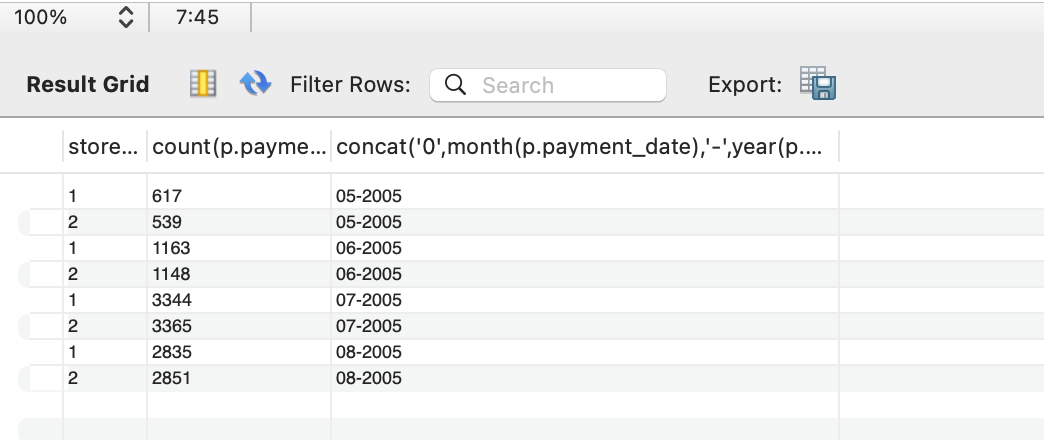
\includegraphics[width=0.75\textwidth]{res/Q8.png}
    \caption{Results of SQL Query for Actors with 'gen' in Last Name}
    \label{fig:actors_with_gen}
\end{figure}


\begin{enumerate}
\def\labelenumi{\arabic{enumi}.}
\setcounter{enumi}{8}
\tightlist
\item
  Trouvez le titre du film, le nom du client, le numéro de téléphone du
  client et l'adresse du client pour tous les DVD en circulation (qui
  n'ont pas prévu d'être rendus)
\end{enumerate}

\begin{Shaded}
\begin{Highlighting}[]
\KeywordTok{select} \KeywordTok{distinct}\NormalTok{ f.title, }\FunctionTok{concat}\NormalTok{(c.first\_name, }\StringTok{\textquotesingle{} \textquotesingle{}}\NormalTok{, c.last\_name) }\KeywordTok{as}\NormalTok{ name, a.phone, }\FunctionTok{concat}\NormalTok{(a.address, }\StringTok{\textquotesingle{} \textquotesingle{}}\NormalTok{, a.district, }\StringTok{\textquotesingle{} \textquotesingle{}}\NormalTok{, a.postal\_code, }\StringTok{\textquotesingle{} \textquotesingle{}}\NormalTok{, ci.city, }\StringTok{\textquotesingle{} \textquotesingle{}}\NormalTok{, co.country) }\KeywordTok{as}\NormalTok{ address}
\KeywordTok{from}\NormalTok{ sakila.rental r}
    \KeywordTok{join}\NormalTok{ sakila.customer c }
        \KeywordTok{on}\NormalTok{ r.customer\_id }\OperatorTok{=}\NormalTok{ c.customer\_id}
    \KeywordTok{join}\NormalTok{ sakila.address a}
        \KeywordTok{on}\NormalTok{ a.address\_id }\OperatorTok{=}\NormalTok{ c.address\_id}
    \KeywordTok{join}\NormalTok{ sakila.inventory i}
        \KeywordTok{on}\NormalTok{ i.inventory\_id }\OperatorTok{=}\NormalTok{ r.inventory\_id}
    \KeywordTok{join}\NormalTok{ sakila.film f}
        \KeywordTok{on}\NormalTok{ f.film\_id }\OperatorTok{=}\NormalTok{ i.film\_id}
    \KeywordTok{join}\NormalTok{ sakila.city ci }
        \KeywordTok{on}\NormalTok{ ci.city\_id }\OperatorTok{=}\NormalTok{ a.city\_id}
    \KeywordTok{join}\NormalTok{ sakila.country co}
        \KeywordTok{on}\NormalTok{ co.country\_id }\OperatorTok{=}\NormalTok{ ci.country\_id}
\KeywordTok{where}\NormalTok{ r.return\_date }\KeywordTok{is} \KeywordTok{null}\NormalTok{;}
\end{Highlighting}
\end{Shaded}


\begin{figure}[H] % Use [H] to enforce positioning
    \centering
    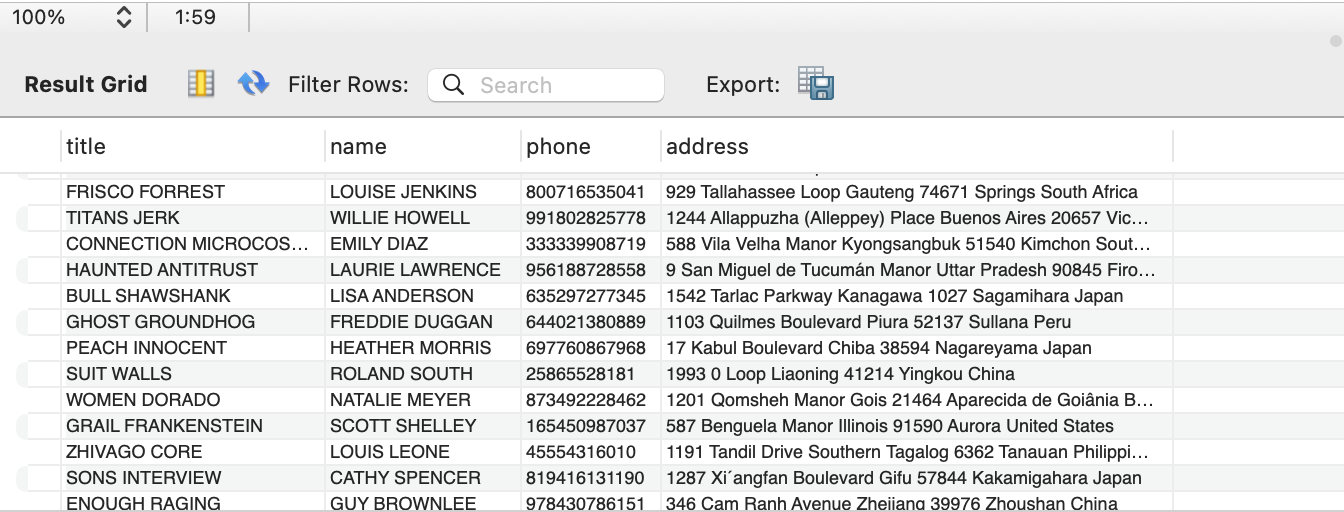
\includegraphics[width=0.75\textwidth]{res/Q9.png}
    \caption{Results of SQL Query for Actors with 'gen' in Last Name}
    \label{fig:actors_with_gen}
\end{figure}


\section{2è partie -- Test technique (type
Entreprise)}\label{uxe8-partie-test-technique-type-entreprise}

\begin{enumerate}
\def\labelenumi{\arabic{enumi}.}
\item
  How can SQL queries be optimized ?

  12 best practices :

  \begin{itemize}
  \tightlist
  \item
    Use indexes effectively
  \item
    Avoid \texttt{SELECT\ *} and retrieve only necessary columns
  \item
    Optimize \texttt{JOIN} operations
  \item
    Minimize the use of subqueries
  \item
    Avoid redundant or unnecessary data retrieval
  \item
    Utilize stored procedures
  \item
    Consider partitioning and sharding
  \item
    Normalize database tables
  \item
    Monitor query performance
  \item
    Use \texttt{UNION\ ALL} instead of \texttt{UNION}
  \item
    Optimize subquery performance
  \item
    Leverage cloud database-specific features
  \end{itemize}
\item
  How do you remove duplicate rows from a table ?

  \begin{itemize}
  \item
    \textbf{Method 1 :} Run the following script :

\begin{Shaded}
\begin{Highlighting}[]
\KeywordTok{SELECT} \KeywordTok{DISTINCT} \OperatorTok{*}
\KeywordTok{INTO}\NormalTok{ duplicate\_table}
\KeywordTok{FROM}\NormalTok{ original\_table}
\KeywordTok{GROUP} \KeywordTok{BY}\NormalTok{ key\_value}
\KeywordTok{HAVING} \FunctionTok{COUNT}\NormalTok{(key\_value) }\OperatorTok{\textgreater{}} \DecValTok{1}

\KeywordTok{DELETE}\NormalTok{ original\_table}
\KeywordTok{WHERE}\NormalTok{ key\_value}
\KeywordTok{IN}\NormalTok{ (}\KeywordTok{SELECT}\NormalTok{ key\_value}
\KeywordTok{FROM}\NormalTok{ duplicate\_table)}

\KeywordTok{INSERT}\NormalTok{ original\_table}
\KeywordTok{SELECT} \OperatorTok{*}
\KeywordTok{FROM}\NormalTok{ duplicate\_table}

\KeywordTok{DROP} \KeywordTok{TABLE}\NormalTok{ duplicate\_table}
\end{Highlighting}
\end{Shaded}

    This script takes the following actions in the given order:

    \begin{itemize}
    \tightlist
    \item
      Moves one instance of any duplicate row in the original table to a
      duplicate table.
    \item
      Deletes all rows from the original table that are also located in
      the duplicate table.
    \item
      Moves the rows in the duplicate table back into the original
      table.
    \item
      Drops the duplicate table.
    \end{itemize}
  \item
    \textbf{Method 2 :} The \texttt{ROW\_NUMBER} function that was
    introduced in Microsoft SQL Server 2005 makes this operation much
    simpler:

\begin{Shaded}
\begin{Highlighting}[]
\KeywordTok{DELETE}\NormalTok{ T}
\KeywordTok{FROM}
\NormalTok{(}
\KeywordTok{SELECT} \OperatorTok{*}
\NormalTok{, DupRank }\OperatorTok{=} \FunctionTok{ROW\_NUMBER}\NormalTok{() }\KeywordTok{OVER}\NormalTok{ (}
            \KeywordTok{PARTITION} \KeywordTok{BY}\NormalTok{ key\_value}
            \KeywordTok{ORDER} \KeywordTok{BY}\NormalTok{ (}\KeywordTok{SELECT} \KeywordTok{NULL}\NormalTok{)}
\NormalTok{            )}
\KeywordTok{FROM}\NormalTok{ original\_table}
\NormalTok{) }\KeywordTok{AS}\NormalTok{ T}
\KeywordTok{WHERE}\NormalTok{ DupRank }\OperatorTok{\textgreater{}} \DecValTok{1}
\end{Highlighting}
\end{Shaded}
  \item
    \textbf{OTHER METHODS:}

    \begin{itemize}
    \item
      SQL delete duplicate Rows using Group By and Having clause
      --\textgreater{} Use the SQL GROUP BY clause to identify the
      duplicate rows. The Group By clause groups data as per the defined
      columns and we can use the COUNT function to check the occurrence
      of a row;
    \item
      SQL delete duplicate Rows using Common Table Expressions (CTE)
      --\textgreater{} Use Common Table Expressions commonly known as
      CTE to remove duplicate rows in SQL Server. It is available
      starting from SQL Server 2005;
    \item
      RANK function to SQL delete duplicate rows --\textgreater{} Use
      the SQL RANK function to remove the duplicate rows as well. SQL
      RANK function gives unique row ID for each row irrespective of the
      duplicate row;
    \item
      Use SSIS package to SQL delete duplicate rows --\textgreater{} Use
      Sort Operator in an SSIS package for removing duplicating rows.
    \end{itemize}
  \end{itemize}
\item
  What are the main differences between HAVING and WHERE SQL clauses ?

  The main difference between WHERE and HAVING clause is that the WHERE
  clause allows you to filter data from specific rows (individual rows)
  from a table based on certain conditions.

  In contrast, the HAVING clause allows you to filter data from a group
  of rows in a query based on conditions involving aggregate values.

  \begin{longtable}[]{@{}
    >{\raggedright\arraybackslash}p{(\columnwidth - 2\tabcolsep) * \real{0.5000}}
    >{\raggedright\arraybackslash}p{(\columnwidth - 2\tabcolsep) * \real{0.5000}}@{}}
  \toprule\noalign{}
  \begin{minipage}[b]{\linewidth}\raggedright
  Where
  \end{minipage} & \begin{minipage}[b]{\linewidth}\raggedright
  Having
  \end{minipage} \\
  \midrule\noalign{}
  \endhead
  \bottomrule\noalign{}
  \endlastfoot
  filters by each row & filters by each group \\
  processed before any grouping & processed after any grouping \\
  cannot have aggregate functions & can have aggregate functions \\
  can be used in SELECT, INSERT, UPDATE, DELETE statements & can only be
  used in SELECT statements \\
  written before GROUP BY clause & written after GROUP BY clause \\
  \end{longtable}
\item
  What is the difference between normalization and denormalization ?

  The goal of normalization is to minimize data redundancy and
  dependency by organizing data into well-structured tables.

  Denormalization involves combining tables that have been normalized to
  improve query performance and simplify data retrieval.

  \begin{longtable}[]{@{}
    >{\raggedright\arraybackslash}p{(\columnwidth - 4\tabcolsep) * \real{0.3333}}
    >{\raggedright\arraybackslash}p{(\columnwidth - 4\tabcolsep) * \real{0.3333}}
    >{\raggedright\arraybackslash}p{(\columnwidth - 4\tabcolsep) * \real{0.3333}}@{}}
  \toprule\noalign{}
  \begin{minipage}[b]{\linewidth}\raggedright
  \end{minipage} & \begin{minipage}[b]{\linewidth}\raggedright
  Normalization
  \end{minipage} & \begin{minipage}[b]{\linewidth}\raggedright
  Denormalization
  \end{minipage} \\
  \midrule\noalign{}
  \endhead
  \bottomrule\noalign{}
  \endlastfoot
  Implementation & Decomposes data into different tables to reduce
  redundancy & Combines data to improve the access time \\
  Query execution speed & Speed of update, delete and write operations
  is higher & Speed of read operations is higher, but that of update and
  write operations is slower \\
  Memory consumption & Memory consumption is less as data redundancy is
  less & Memory consumption is more as redundancy is introduced \\
  Number of tables & Number of tables is more on account of
  decomposition of data & Combines data and hence number of tables are
  less \\
  Data integrity & Data integrity is maintained & Data integrity might
  not be maintained \\
  \end{longtable}
\item
  What are the key differences between the DELETE and TRUNCATE SQL
  commands ?

  DELETE is a SQL command that removes one or multiple rows from a table
  using conditions.

  TRUNCATE is a SQL command that removes all the rows from a table
  without using any condition.

  \begin{longtable}[]{@{}
    >{\raggedright\arraybackslash}p{(\columnwidth - 2\tabcolsep) * \real{0.5000}}
    >{\raggedright\arraybackslash}p{(\columnwidth - 2\tabcolsep) * \real{0.5000}}@{}}
  \toprule\noalign{}
  \begin{minipage}[b]{\linewidth}\raggedright
  Truncate
  \end{minipage} & \begin{minipage}[b]{\linewidth}\raggedright
  Delete
  \end{minipage} \\
  \midrule\noalign{}
  \endhead
  \bottomrule\noalign{}
  \endlastfoot
  It removes all rows from a table + faster + does not use as much undo
  space as a delete & It is used to remove rows from table. A WHERE
  clause can be used to only remove some rows \\
  It is a DDL command so this command change structure of table & It is
  a DML command. It only remove rows from a table, leaving the table
  structure untouched \\
  You cannot rollback in Truncate & In DELETE, you can rollback \\
  In SQL, the auto increment counter gets reset with truncate & The auto
  increment counter cannot get reset with delete \\
  \end{longtable}
\item
  What are some ways to prevent duplicate entries when making a query?

  To prevent duplicate entries when making a query, you can consider the
  following approaches:

  \begin{enumerate}
  \def\labelenumii{\arabic{enumii}.}
  \tightlist
  \item
    \textbf{Use \texttt{DISTINCT}}: When selecting data from a database,
    include the \texttt{DISTINCT} keyword in your SQL query. This will
    return only unique rows based on the columns you specify.
  \end{enumerate}

\begin{Shaded}
\begin{Highlighting}[]
\KeywordTok{SELECT} \KeywordTok{DISTINCT}\NormalTok{ column1, column2 }\KeywordTok{FROM}\NormalTok{ table\_name;}
\end{Highlighting}
\end{Shaded}

  \begin{enumerate}
  \def\labelenumii{\arabic{enumii}.}
  \setcounter{enumii}{1}
  \tightlist
  \item
    \textbf{Use Grouping}: Utilize the \texttt{GROUP\ BY} clause to
    group records by specific columns. This will aggregate results and
    can be combined with aggregate functions to eliminate duplicates.
  \end{enumerate}

\begin{Shaded}
\begin{Highlighting}[]
\KeywordTok{SELECT}\NormalTok{ column1, }\FunctionTok{COUNT}\NormalTok{(}\OperatorTok{*}\NormalTok{) }\KeywordTok{FROM}\NormalTok{ table\_name }\KeywordTok{GROUP} \KeywordTok{BY}\NormalTok{ column1;}
\end{Highlighting}
\end{Shaded}

  \begin{enumerate}
  \def\labelenumii{\arabic{enumii}.}
  \setcounter{enumii}{2}
  \item
    \textbf{Implement Primary Keys and Unique Constraints}: In your
    database schema, define primary keys and unique constraints on
    columns where duplicates should not occur. This will automatically
    prevent the insertion of duplicate records.
  \item
    \textbf{Use \texttt{JOIN} with Care}: When joining tables, ensure
    you are joining on the correct keys and using appropriate conditions
    to avoid unintended duplication of rows.
  \item
    \textbf{Window Functions}: Use window functions to rank or number
    rows based on specific criteria, then filter out duplicates based on
    that ranking.
  \end{enumerate}

\begin{Shaded}
\begin{Highlighting}[]
\KeywordTok{SELECT} \OperatorTok{*} \KeywordTok{FROM}\NormalTok{ (}
    \KeywordTok{SELECT} \OperatorTok{*}\NormalTok{, }\FunctionTok{ROW\_NUMBER}\NormalTok{() }\KeywordTok{OVER}\NormalTok{ (}\KeywordTok{PARTITION} \KeywordTok{BY}\NormalTok{ column1 }\KeywordTok{ORDER} \KeywordTok{BY}\NormalTok{ column2) }\KeywordTok{as}\NormalTok{ rn}
    \KeywordTok{FROM}\NormalTok{ table\_name}
\NormalTok{) }\KeywordTok{AS}\NormalTok{ temp}
\KeywordTok{WHERE}\NormalTok{ rn }\OperatorTok{=} \DecValTok{1}\NormalTok{;}
\end{Highlighting}
\end{Shaded}
\item
  What are the different types of relationships in SQL?

  In SQL and relational database design, there are three main types of
  relationships that define how tables are related to each other:

  \begin{enumerate}
  \def\labelenumii{\arabic{enumii}.}
  \item
    \textbf{One-to-One (1:1)}:

    \begin{itemize}
    \tightlist
    \item
      In a one-to-one relationship, a row in one table is linked to a
      single row in another table, and vice versa.
    \item
      This type of relationship is often used to split a table for
      normalization or to separate optional data.
    \item
      \textbf{Example}: A \texttt{Users} table and a
      \texttt{UserProfiles} table, where each user has exactly one
      profile.
    \end{itemize}
  \item
    \textbf{One-to-Many (1:N)}:

    \begin{itemize}
    \tightlist
    \item
      In a one-to-many relationship, a row in one table can be
      associated with multiple rows in another table, but a row in the
      second table is linked to only one row in the first table.
    \item
      This is the most common type of relationship in relational
      databases.
    \item
      \textbf{Example}: A \texttt{Customers} table and an
      \texttt{Orders} table, where each customer can have multiple
      orders, but each order is associated with only one customer.
    \end{itemize}
  \item
    \textbf{Many-to-Many (M:N)}:

    \begin{itemize}
    \tightlist
    \item
      In a many-to-many relationship, multiple rows in one table can be
      related to multiple rows in another table. This type of
      relationship requires a junction (or linking) table to facilitate
      the relationship.
    \item
      \textbf{Example}: A \texttt{Students} table and a \texttt{Courses}
      table, where a student can enroll in multiple courses, and a
      course can have multiple students. A junction table called
      \texttt{Enrollments} could be created to link students and
      courses.
    \end{itemize}
  \item
    \textbf{Additional Concepts}:

    \begin{itemize}
    \item
      \textbf{Self-Referencing Relationships}: A table may relate to
      itself in a one-to-one or one-to-many manner. For example, an
      \texttt{Employees} table where each employee can have a manager
      who is also an employee.
    \item
      \textbf{Foreign Keys}: Relationships are typically enforced using
      foreign keys, which are fields in one table that refer to the
      primary key of another table. This ensures referential integrity.
    \end{itemize}
  \end{enumerate}
\item
  SQL code example + Queries :

  \begin{enumerate}
  \def\labelenumii{\arabic{enumii}.}
  \item
    Give an example of the SQL code that will insert the `Input data'
    into the two tables. You must ensure that the student table includes
    the correct {[}dbo{]}.{[}Master{]}.{[}id{]} in the
    {[}dbo{]}.{[}student{]}.{[}Master\_id{]} column.

\begin{Shaded}
\begin{Highlighting}[]
\KeywordTok{with}\NormalTok{ new\_master }\KeywordTok{as}\NormalTok{ (}
    \KeywordTok{insert} \KeywordTok{into}\NormalTok{ [dbo].[}\KeywordTok{Master}\NormalTok{] (name, some\_column)}
    \KeywordTok{values}\NormalTok{ (}\StringTok{\textquotesingle{}Example Name\textquotesingle{}}\NormalTok{, }\StringTok{\textquotesingle{}Example Value\textquotesingle{}}\NormalTok{)}
\NormalTok{    output inserted.}\KeywordTok{id}
\NormalTok{)}
\KeywordTok{insert} \KeywordTok{into}\NormalTok{ [dbo].[student] (Master\_id, student\_name, student\_column)}
\KeywordTok{select} \KeywordTok{id}\NormalTok{, }\StringTok{\textquotesingle{}Student Name\textquotesingle{}}\NormalTok{, }\StringTok{\textquotesingle{}Student Value\textquotesingle{}}
\KeywordTok{from}\NormalTok{ new\_master;}
\end{Highlighting}
\end{Shaded}
  \item
    SQL code that shows courses', subject names and the number of
    students taking the course only if the course has three or more
    students on the course.

\begin{Shaded}
\begin{Highlighting}[]
\KeywordTok{select}\NormalTok{ sub.}\OperatorTok{*}\NormalTok{, }\FunctionTok{count}\NormalTok{(stu.subject\_id) }\KeywordTok{as}\NormalTok{ nb\_stu\_enrolled}
\KeywordTok{from}\NormalTok{ Q8\_SDA.student stu}
    \KeywordTok{join}\NormalTok{ Q8\_SDA.subject sub}
        \KeywordTok{on}\NormalTok{ stu.subject\_id }\OperatorTok{=}\NormalTok{ sub.subject\_id}
\KeywordTok{group} \KeywordTok{by}\NormalTok{ stu.subject\_id}
\KeywordTok{order} \KeywordTok{by}\NormalTok{ stu.subject\_id }\KeywordTok{asc}\NormalTok{;}
\end{Highlighting}
\end{Shaded}
  \end{enumerate}

\begin{figure}[H] % Use [H] to enforce positioning
    \centering
    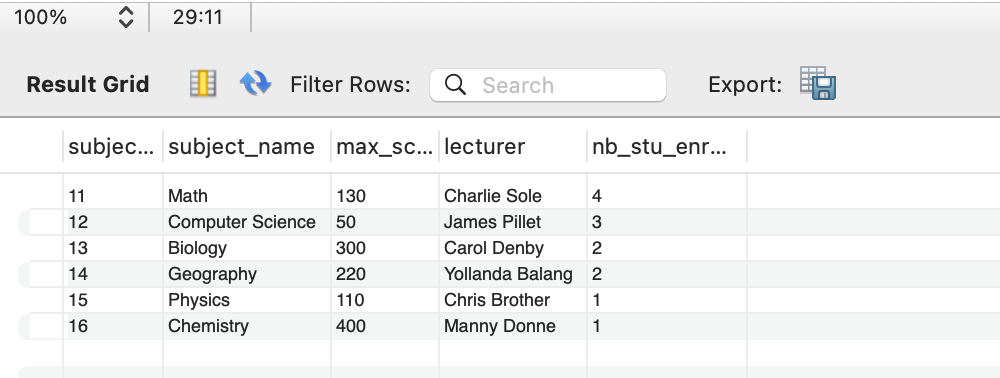
\includegraphics[width=0.75\textwidth]{res/Q8-2.png}
    \caption{Results of SQL Query for Actors with 'gen' in Last Name}
    \label{fig:actors_with_gen}
\end{figure}

  
\item
  2 parts :

  \textbf{HYPOTHESIS} :

  \begin{itemize}
  \tightlist
  \item
    Total = \texttt{Orders.total}
  \item
    Total \emph{from the orders table} = Total amount spent \emph{(by
    each customer from the orders table)} =
    \texttt{sum((OrderItems.price\ *\ OrderItems.quantity))}
  \end{itemize}

  \begin{enumerate}
  \def\labelenumii{\arabic{enumii}.}
  \item
    Retrieve the order\_id , customer\_id, and total from the orders
    table where the \textbf{total} is greater than 400

\begin{Shaded}
\begin{Highlighting}[]
\KeywordTok{select}\NormalTok{ o.order\_id, o.customer\_id, }\FunctionTok{sum}\NormalTok{((i.price }\OperatorTok{*}\NormalTok{ i.quantity)) }\KeywordTok{as}\NormalTok{ total\_from\_orders\_table}
\KeywordTok{from}\NormalTok{ orders o}
    \KeywordTok{join}\NormalTok{ order\_items i }
        \KeywordTok{on}\NormalTok{ o.order\_id }\OperatorTok{=}\NormalTok{ i.order\_id}
\KeywordTok{where}\NormalTok{ o.total }\OperatorTok{\textgreater{}} \DecValTok{400}
\KeywordTok{group} \KeywordTok{by}\NormalTok{ o.order\_id;}
\end{Highlighting}
\end{Shaded}

\begin{figure}[H] % Use [H] to enforce positioning
    \centering
    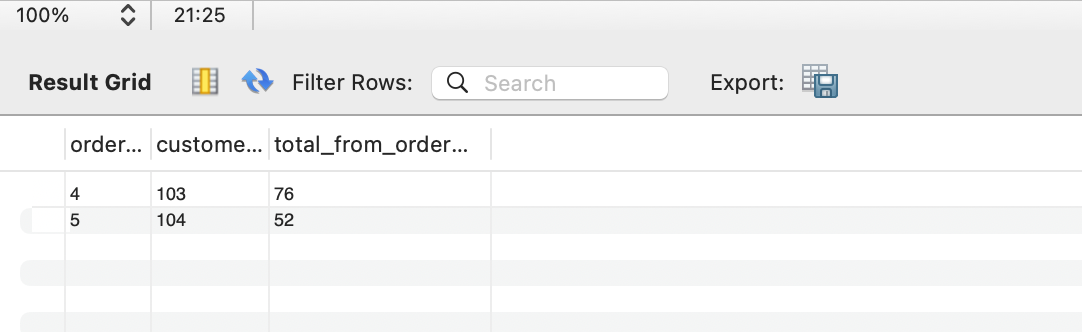
\includegraphics[width=0.75\textwidth]{res/Q9-1.png}
    \caption{Results of SQL Query for Actors with 'gen' in Last Name}
    \label{fig:actors_with_gen}
\end{figure}

  \item
    Retrieve the customer\_id and the \textbf{total amount spent} by
    each customer from the orders table, ordered by the \textbf{total
    amount spent} in descending order

\begin{Shaded}
\begin{Highlighting}[]
\KeywordTok{select}\NormalTok{ o.customer\_id, }\FunctionTok{sum}\NormalTok{((i.price }\OperatorTok{*}\NormalTok{ i.quantity)) }\KeywordTok{as}\NormalTok{ total\_from\_orders\_table}
\KeywordTok{from}\NormalTok{ orders o}
    \KeywordTok{join}\NormalTok{ order\_items i }
        \KeywordTok{on}\NormalTok{ o.order\_id }\OperatorTok{=}\NormalTok{ i.order\_id}
\KeywordTok{group} \KeywordTok{by}\NormalTok{ o.order\_id}
\KeywordTok{order} \KeywordTok{by}\NormalTok{ o.total }\KeywordTok{desc}\NormalTok{;}
\end{Highlighting}
\end{Shaded}
  \end{enumerate}

\begin{figure}[H] % Use [H] to enforce positioning
    \centering
    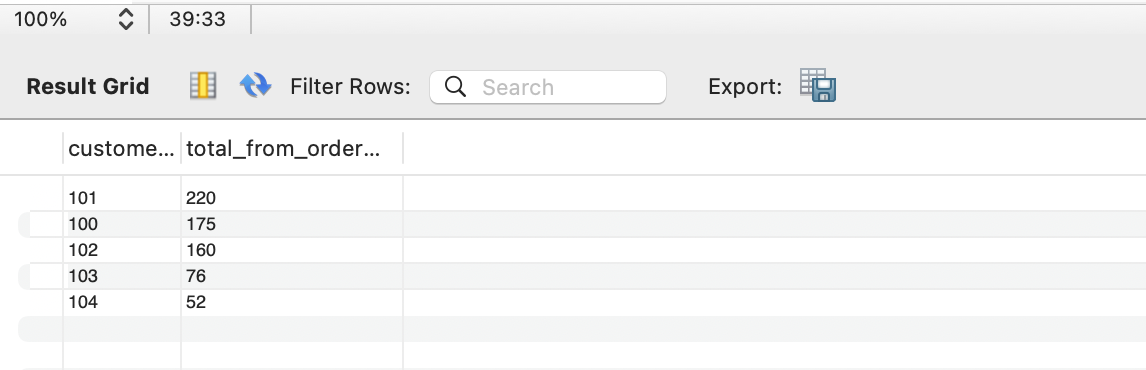
\includegraphics[width=0.75\textwidth]{res/Q9-2.png}
    \caption{Results of SQL Query for Actors with 'gen' in Last Name}
    \label{fig:actors_with_gen}
\end{figure}

  
\item
  Write a query that shows the total quantity sold for each product.

\begin{Shaded}
\begin{Highlighting}[]
\KeywordTok{select}\NormalTok{ o.product\_id, }\FunctionTok{sum}\NormalTok{(o.quantity) }\KeywordTok{as}\NormalTok{ total\_quantity\_sold}
\KeywordTok{from}\NormalTok{ order\_items\_v2 o}
\KeywordTok{group} \KeywordTok{by}\NormalTok{ o.product\_id;}
\end{Highlighting}
\end{Shaded}

\begin{figure}[H] % Use [H] to enforce positioning
    \centering
    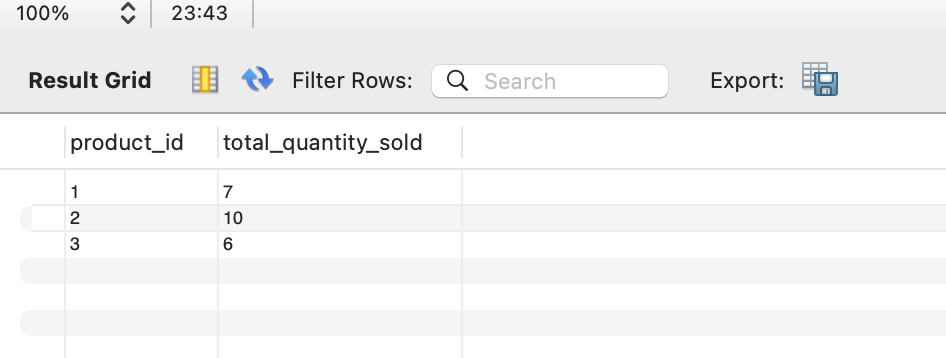
\includegraphics[width=0.75\textwidth]{res/Q10.png}
    \caption{Results of SQL Query for Actors with 'gen' in Last Name}
    \label{fig:actors_with_gen}
\end{figure}


\item
  Database creation + insertion

\begin{Shaded}
\begin{Highlighting}[]
\KeywordTok{create} \KeywordTok{table}\NormalTok{ Customers }
\NormalTok{(}
    \KeywordTok{id} \DataTypeTok{int}\NormalTok{, }
\NormalTok{    name }\DataTypeTok{varchar}\NormalTok{(}\DecValTok{100}\NormalTok{),}
\NormalTok{    address }\DataTypeTok{varchar}\NormalTok{(}\DecValTok{100}\NormalTok{),}
\NormalTok{    city }\DataTypeTok{varchar}\NormalTok{(}\DecValTok{100}\NormalTok{),}
\NormalTok{    country }\DataTypeTok{varchar}\NormalTok{(}\DecValTok{100}\NormalTok{),}

    \KeywordTok{constraint}\NormalTok{ customer\_pk }\KeywordTok{primary} \KeywordTok{key}\NormalTok{(}\KeywordTok{id}\NormalTok{)}
\NormalTok{);}

\KeywordTok{create} \KeywordTok{table}\NormalTok{ Orders}
\NormalTok{(}
    \KeywordTok{id} \DataTypeTok{int}\NormalTok{,}
\NormalTok{    customer\_id }\DataTypeTok{int}\NormalTok{,}
\NormalTok{    order\_date datetime,}
\NormalTok{    total }\DataTypeTok{int}\NormalTok{,}

    \KeywordTok{constraint}\NormalTok{ orders\_pk }\KeywordTok{primary} \KeywordTok{key}\NormalTok{(}\KeywordTok{id}\NormalTok{),}
    \KeywordTok{constraint}\NormalTok{ orders\_cus\_fk }\KeywordTok{foreign} \KeywordTok{key}\NormalTok{(customer\_id)}
        \KeywordTok{references}\NormalTok{ Customers }\KeywordTok{on} \KeywordTok{delete} \KeywordTok{cascade}
\NormalTok{);}

\KeywordTok{create} \KeywordTok{table}\NormalTok{ OrderDetails }
\NormalTok{(}
    \KeywordTok{id} \DataTypeTok{int}\NormalTok{,}
\NormalTok{    order\_id }\DataTypeTok{int}\NormalTok{,}
\NormalTok{    product }\DataTypeTok{varchar}\NormalTok{(}\DecValTok{100}\NormalTok{),}
\NormalTok{    quantity }\DataTypeTok{int}\NormalTok{,}
\NormalTok{    price }\DataTypeTok{float}\NormalTok{,}

    \KeywordTok{constraint}\NormalTok{ order\_details\_pk }\KeywordTok{primary} \KeywordTok{key}\NormalTok{(}\KeywordTok{id}\NormalTok{),}
    \KeywordTok{constraint}\NormalTok{ orders\_fk }\KeywordTok{foreign} \KeywordTok{key}\NormalTok{(order\_id)}
        \KeywordTok{references}\NormalTok{ Orders }\KeywordTok{on} \KeywordTok{delete} \KeywordTok{cascade}
\NormalTok{);}



\CommentTok{{-}{-} Insert unique customers into Customers table}
\KeywordTok{insert} \KeywordTok{into}\NormalTok{ Customers (}\KeywordTok{id}\NormalTok{, name, address, city, country)}
\KeywordTok{select} \KeywordTok{distinct}\NormalTok{ customer\_id, customer\_name, customer\_addr, customer\_city, customer\_country}
\KeywordTok{from}\NormalTok{ customer\_orders;}

\CommentTok{{-}{-} Insert orders into Orders table}
\KeywordTok{insert} \KeywordTok{into}\NormalTok{ Orders (}\KeywordTok{id}\NormalTok{, customer\_id, order\_date, total)}
\KeywordTok{select} \KeywordTok{distinct}\NormalTok{ order\_id, customer\_id, order\_date, order\_total}
\KeywordTok{from}\NormalTok{ sdacustomer\_orders}
\KeywordTok{where}\NormalTok{ order\_id }\KeywordTok{is} \KeywordTok{not} \KeywordTok{null}\NormalTok{;}

\CommentTok{{-}{-} Insert order details into OrderDetails table}
\KeywordTok{insert} \KeywordTok{into}\NormalTok{ OrderDetails (}\KeywordTok{id}\NormalTok{, order\_id, product, quantity, price)}
\KeywordTok{select} \KeywordTok{distinct}\NormalTok{ order\_details\_id, order\_id, product, quantity, price}
\NormalTok{frcustomer\_orders}
\KeywordTok{where}\NormalTok{ order\_id }\KeywordTok{is} \KeywordTok{not} \KeywordTok{null}\NormalTok{;}
\end{Highlighting}
\end{Shaded}
\end{enumerate}

\section{References}\label{references}

\begin{enumerate}
\def\labelenumi{\arabic{enumi}.}
\tightlist
\item
  ThoughtSpot. (n.d.). Optimizing SQL queries: A guide to data modeling
  best practices. ThoughtSpot. Retrieved November 1, 2024, from
  https://www.thoughtspot.com/data-trends/data-modeling/optimizing-sql-queries
\item
  SQL Shack. (2021, March 30). Different ways to SQL delete duplicate
  rows from a SQL table. SQL Shack. Retrieved November 1, 2024, from
  https://www.sqlshack.com/different-ways-to-sql-delete-duplicate-rows-from-a-sql-table/
\item
  Microsoft. (n.d.). Remove duplicate rows from a SQL Server table.
  Microsoft Learn. Retrieved November 1, 2024, from
  https://learn.microsoft.com/en-us/troubleshoot/sql/database-engine/development/remove-duplicate-rows-sql-server-tab
\end{enumerate}

    \begin{center}\rule{0.5\linewidth}{0.5pt}\end{center}


    % Add a bibliography block to the postdoc


    
\end{document}